\thispagestyle{scrheadings}
\section{Vergleich mit anderen Hexapoden}
\label{disc-comp}

\begin{figure}[H]
    \centering
    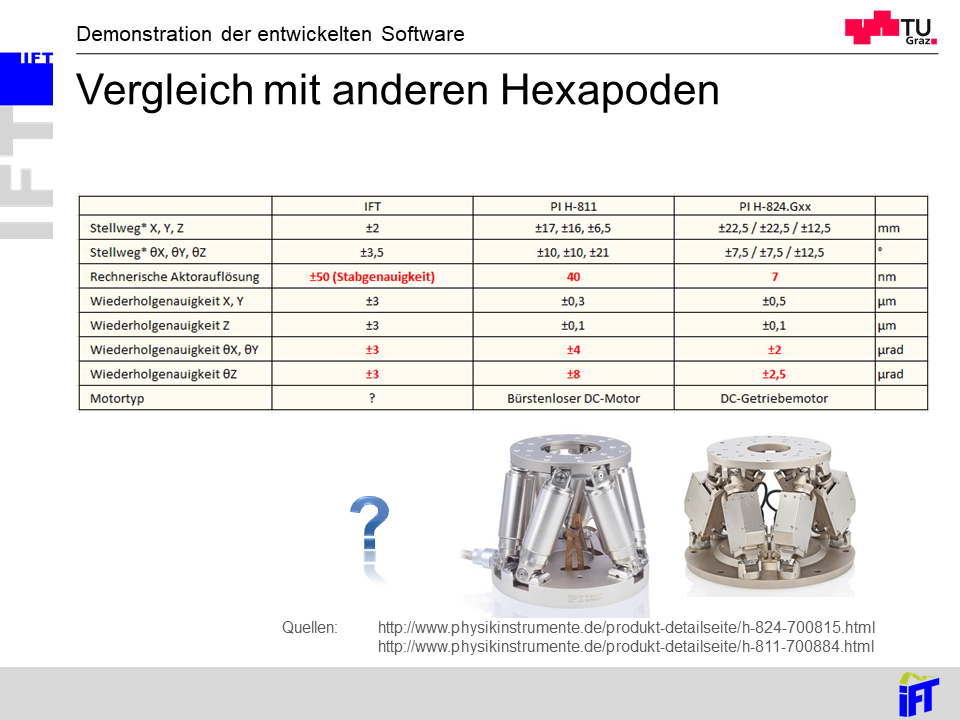
\includegraphics[width=0.7\textwidth]{disc/comp}
    \caption[Folie]{Folie, Quelle: Eigene Darstellung}
    \label{fig:comp}
\end{figure}

\thispagestyle{scrheadings}
\section{Anforderungen an die Messtechnik}
\label{disc-mess}

\begin{figure}[H]
    \centering
    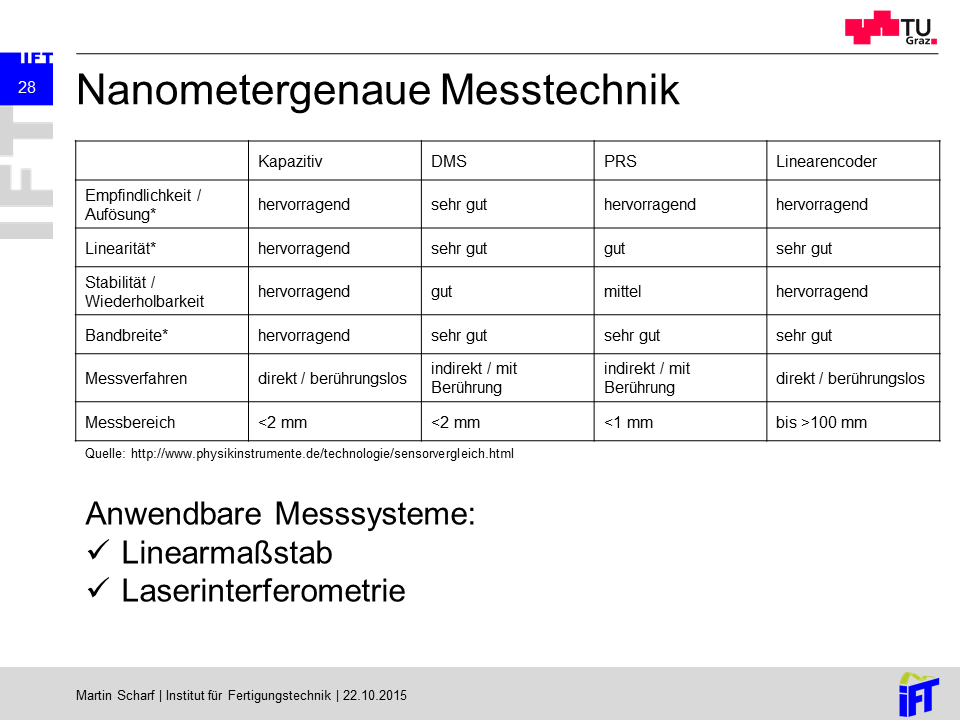
\includegraphics[width=0.7\textwidth]{disc/mess1}
    \caption[Folie]{Folie, Quelle: Eigene Darstellung}
    \label{fig:mess1}
\end{figure}

\begin{figure}[H]
    \centering
    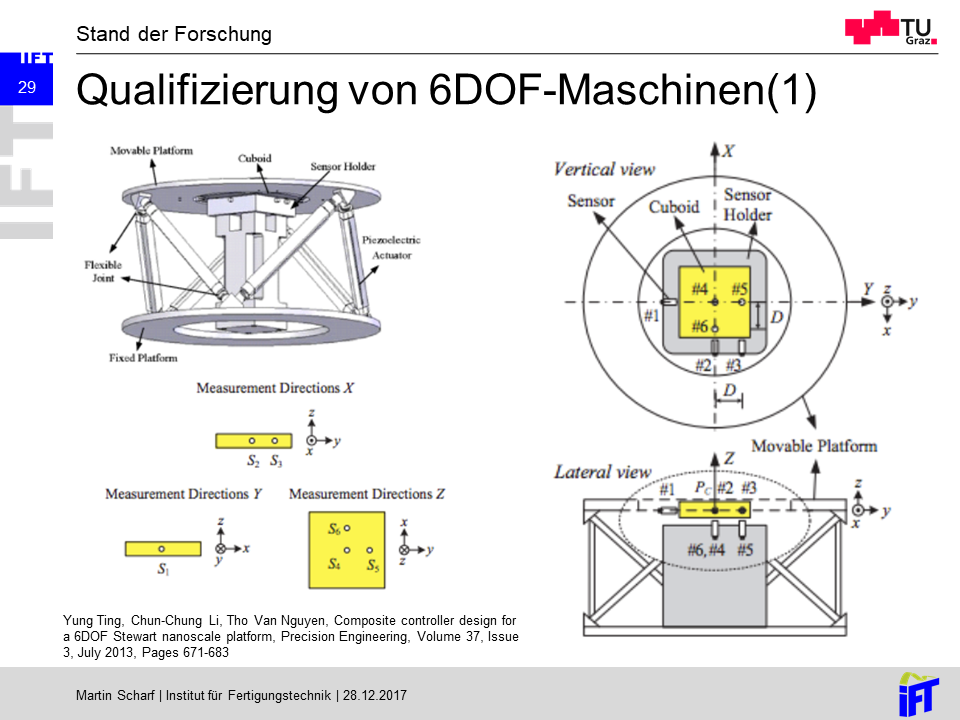
\includegraphics[width=0.7\textwidth]{disc/mess2}
    \caption[Folie]{Folie, Quelle: Eigene Darstellung}
    \label{fig:mess2}
\end{figure}

\begin{figure}[H]
    \centering
    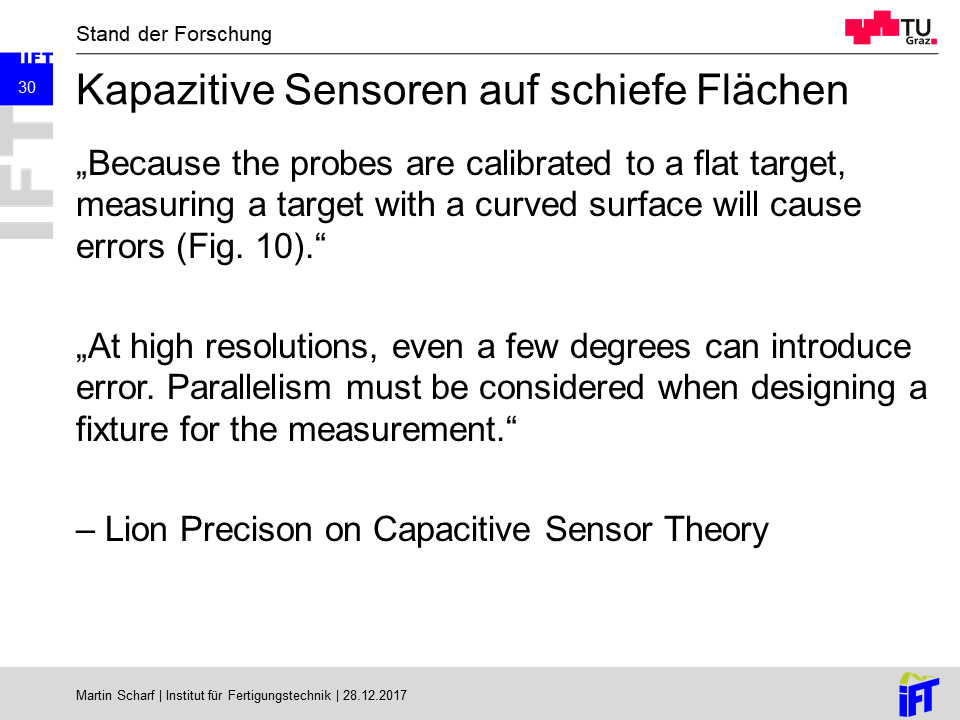
\includegraphics[width=0.7\textwidth]{disc/mess3}
    \caption[Folie]{Folie, Quelle: Eigene Darstellung}
    \label{fig:mess3}
\end{figure}

\begin{figure}[H]
    \centering
    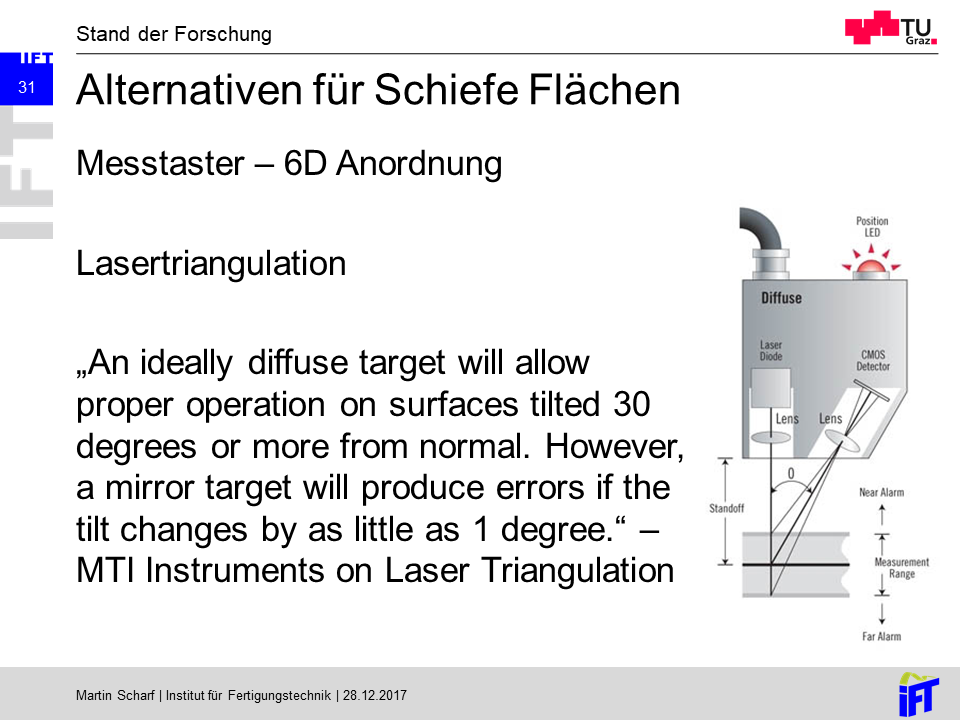
\includegraphics[width=0.7\textwidth]{disc/mess4}
    \caption[Folie]{Folie, Quelle: Eigene Darstellung}
    \label{fig:mess4}
\end{figure}

\begin{figure}[H]
    \centering
    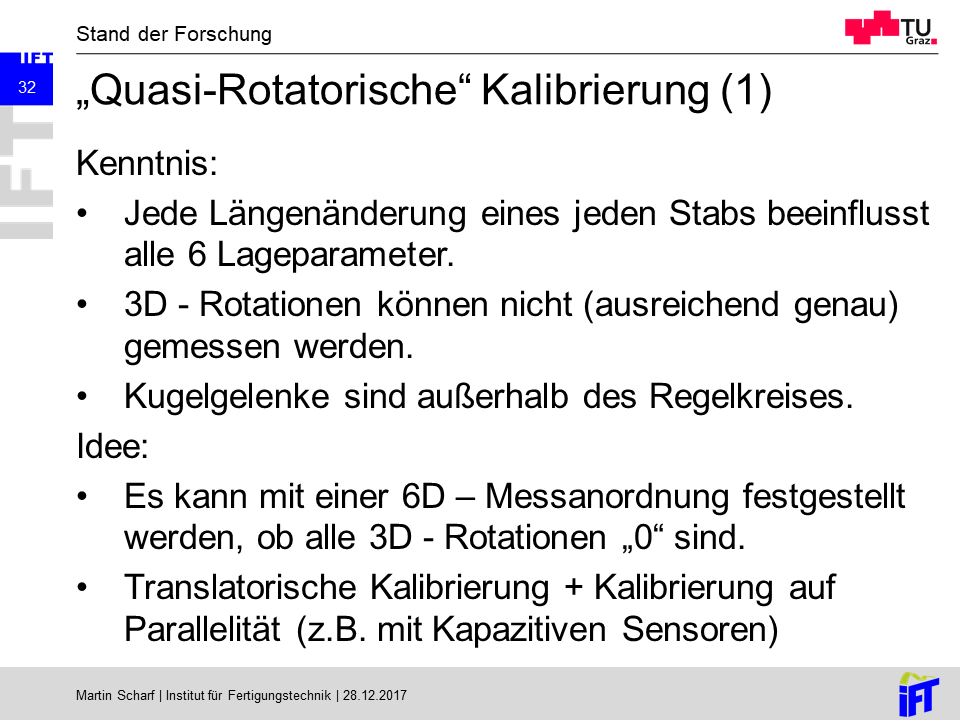
\includegraphics[width=0.7\textwidth]{disc/mess5}
    \caption[Folie]{Folie, Quelle: Eigene Darstellung}
    \label{fig:mess5}
\end{figure}

\begin{figure}[H]
    \centering
    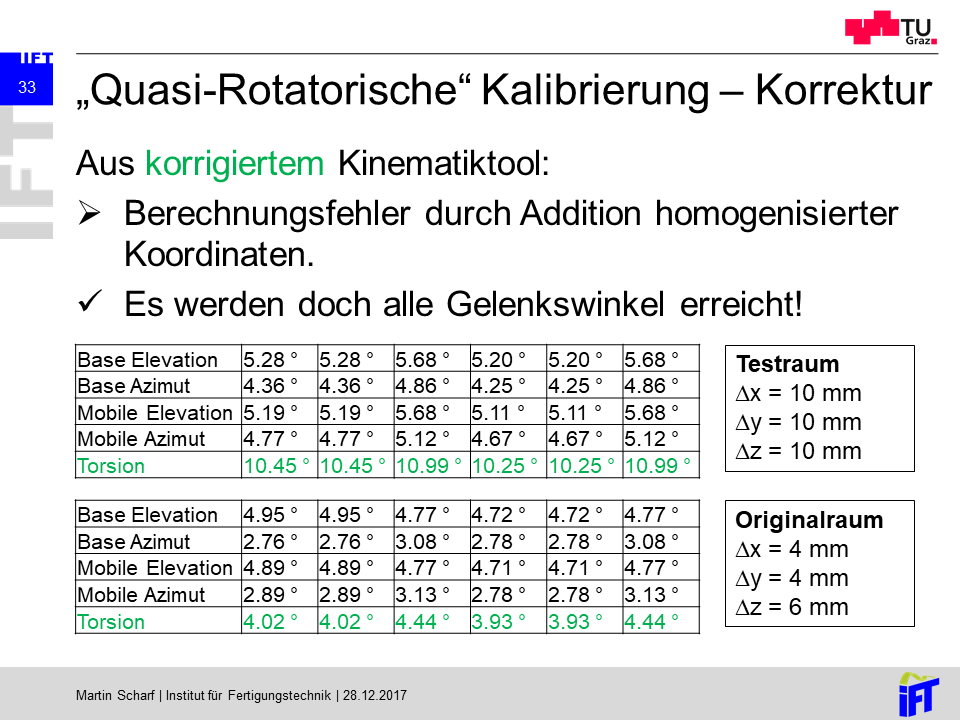
\includegraphics[width=0.7\textwidth]{disc/mess6}
    \caption[Folie]{Folie, Quelle: Eigene Darstellung}
    \label{fig:mess6}
\end{figure}

\begin{figure}[H]
    \centering
    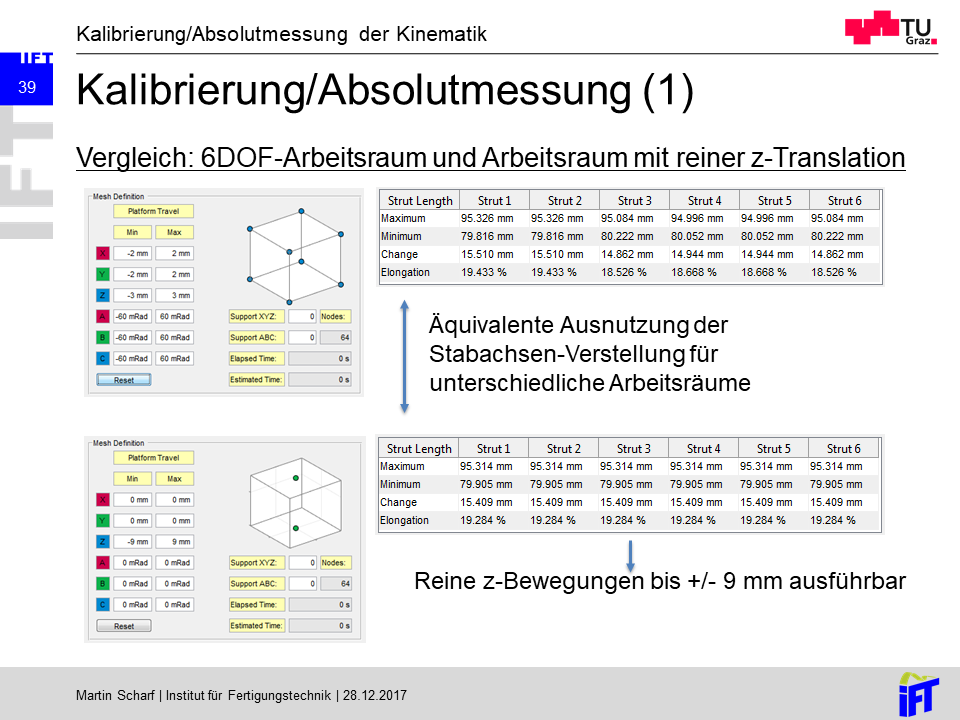
\includegraphics[width=0.7\textwidth]{disc/mess7}
    \caption[Folie]{Folie, Quelle: Eigene Darstellung}
    \label{fig:mess7}
\end{figure}

\begin{figure}[H]
    \centering
    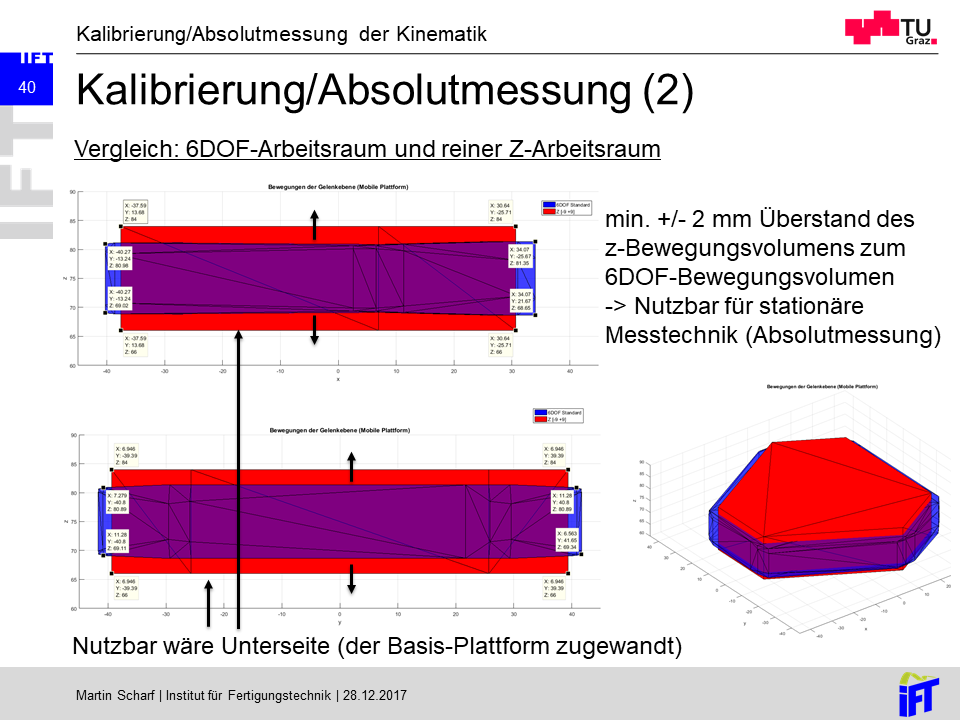
\includegraphics[width=0.7\textwidth]{disc/mess8}
    \caption[Folie]{Folie, Quelle: Eigene Darstellung}
    \label{fig:mess8}
\end{figure}

\begin{figure}[H]
    \centering
    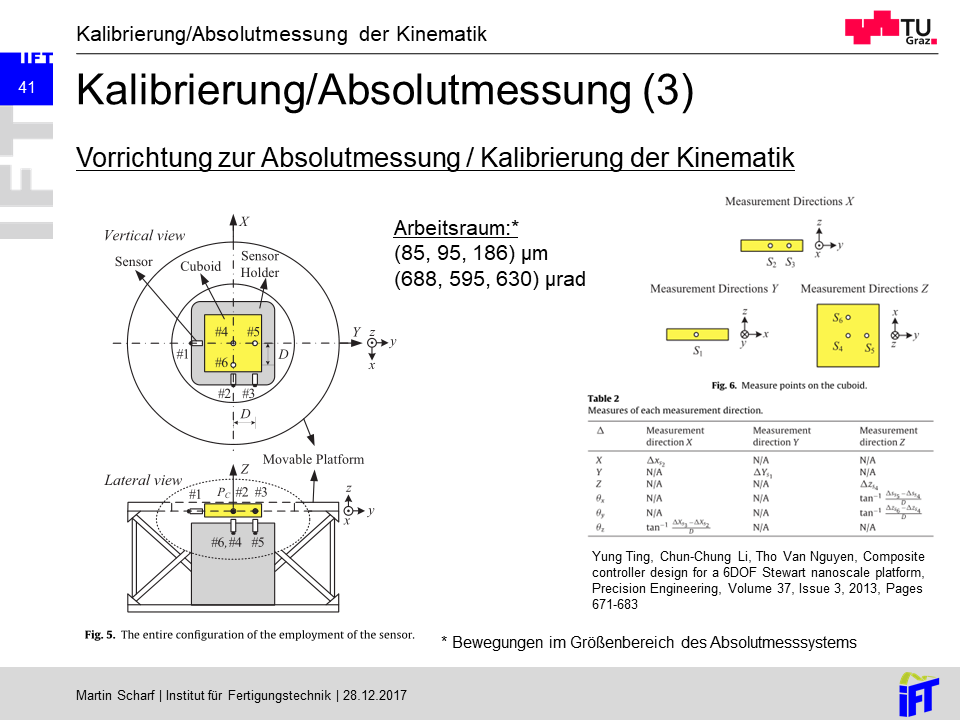
\includegraphics[width=0.7\textwidth]{disc/mess9}
    \caption[Folie]{Folie, Quelle: Eigene Darstellung}
    \label{fig:mess9}
\end{figure}

\thispagestyle{scrheadings}
\section{Werkstoffwahl}
\label{disc-mess}

\begin{figure}[H]
    \centering
    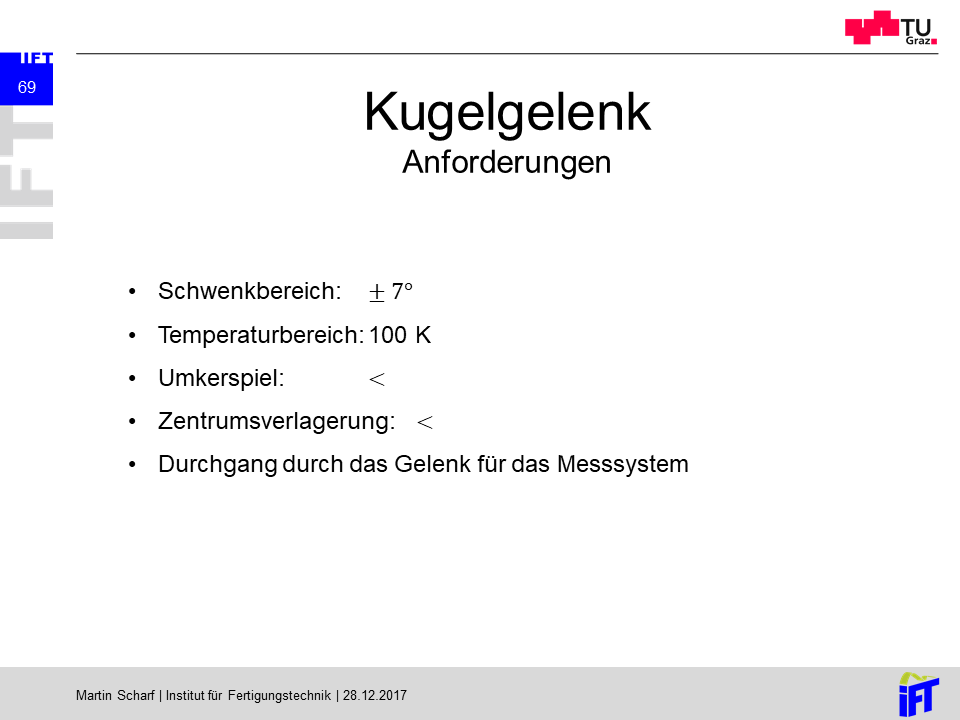
\includegraphics[width=0.7\textwidth]{disc/ws1}
    \caption[Folie]{Folie, Quelle: Eigene Darstellung}
    \label{fig:ws1}
\end{figure}

\begin{figure}[H]
    \centering
    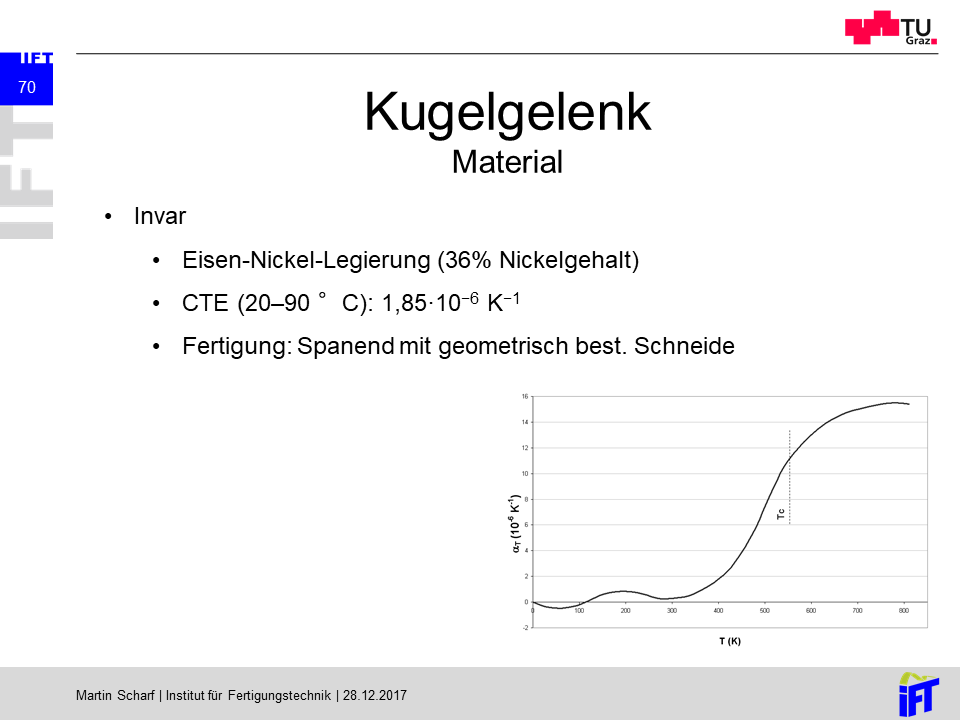
\includegraphics[width=0.7\textwidth]{disc/ws2}
    \caption[Folie]{Folie, Quelle: Eigene Darstellung}
    \label{fig:ws2}
\end{figure}

\begin{figure}[H]
    \centering
    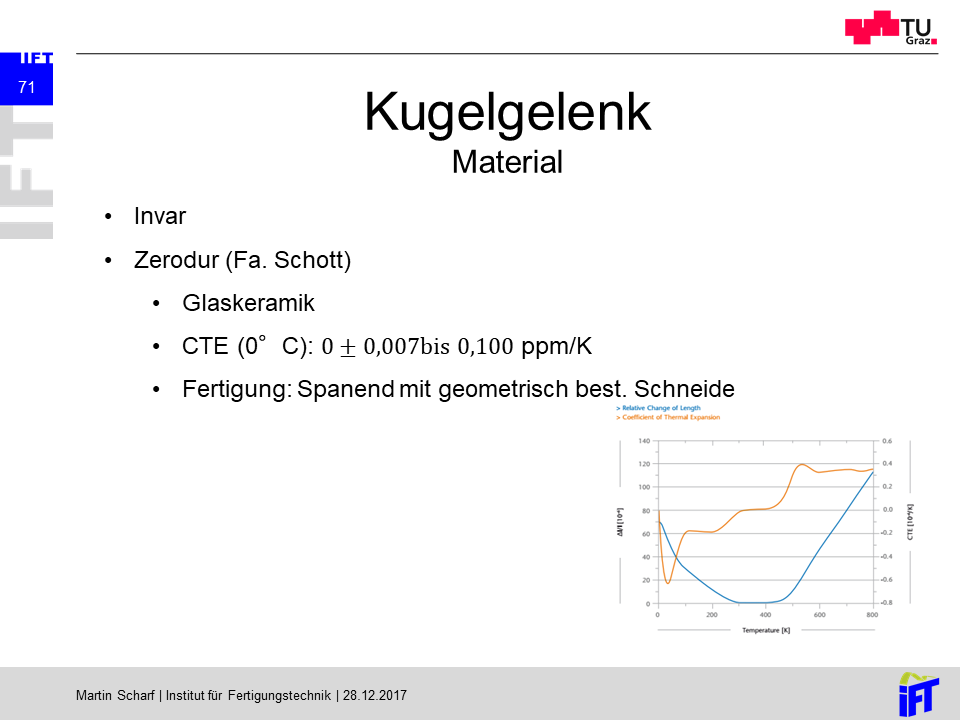
\includegraphics[width=0.7\textwidth]{disc/ws3}
    \caption[Folie]{Folie, Quelle: Eigene Darstellung}
    \label{fig:ws3}
\end{figure}

\begin{figure}[H]
    \centering
    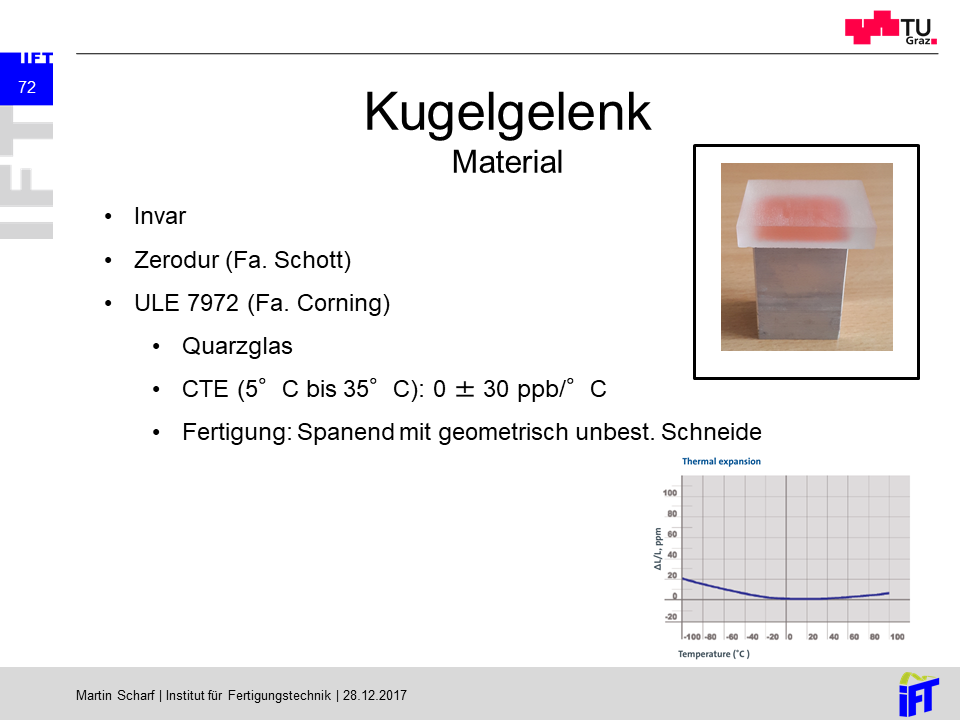
\includegraphics[width=0.7\textwidth]{disc/ws4}
    \caption[Folie]{Folie, Quelle: Eigene Darstellung}
    \label{fig:ws4}
\end{figure}

\begin{figure}[H]
    \centering
    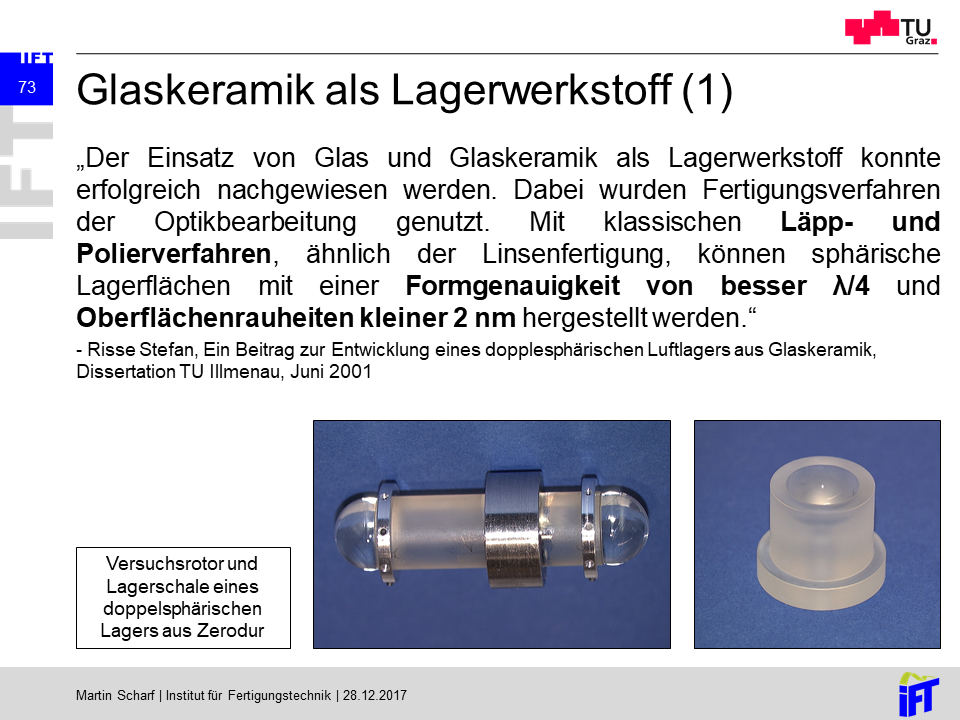
\includegraphics[width=0.7\textwidth]{disc/ws5}
    \caption[Folie]{Folie, Quelle: Eigene Darstellung}
    \label{fig:ws5}
\end{figure}

\begin{figure}[H]
    \centering
    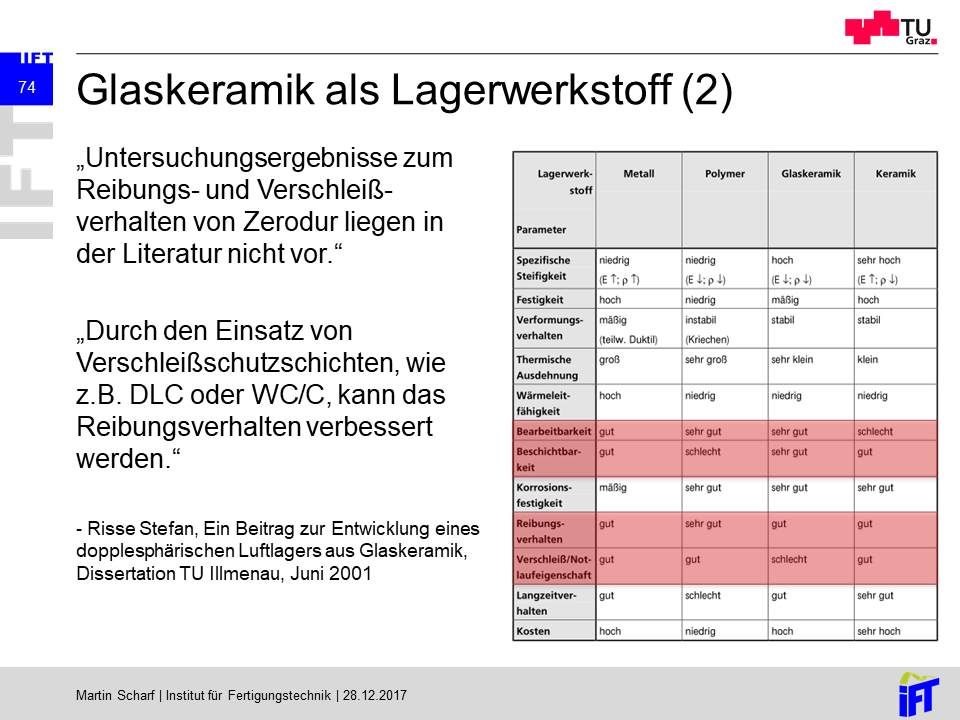
\includegraphics[width=0.7\textwidth]{disc/ws6}
    \caption[Folie]{Folie, Quelle: Eigene Darstellung}
    \label{fig:ws6}
\end{figure}

\begin{figure}[H]
    \centering
    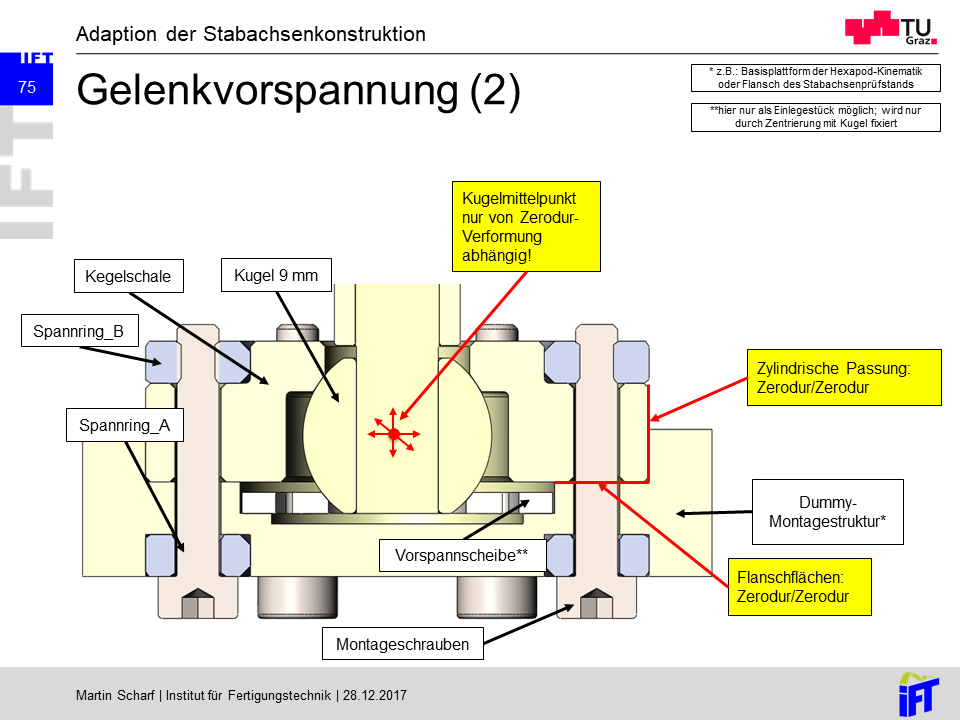
\includegraphics[width=0.7\textwidth]{disc/ws7}
    \caption[Folie]{Folie, Quelle: Eigene Darstellung}
    \label{fig:ws7}
\end{figure}

\thispagestyle{scrheadings}
\section{Anforderungen an die Antriebstechnik}
\label{disc-mess}

\begin{figure}[H]
    \centering
    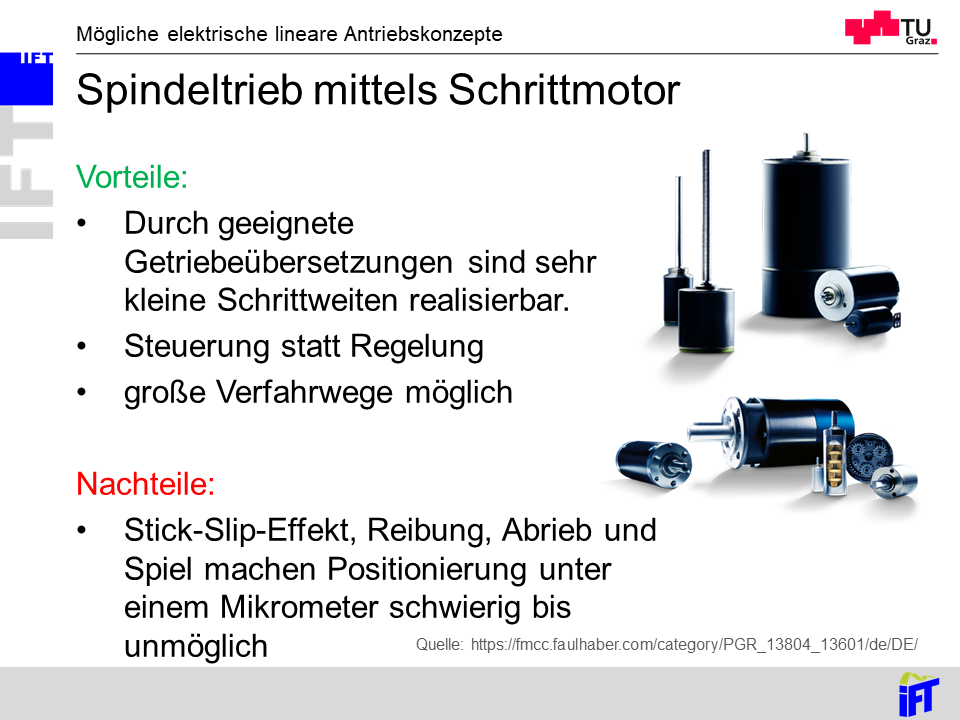
\includegraphics[width=0.7\textwidth]{disc/mech1}
    \caption[Folie]{Folie, Quelle: Eigene Darstellung}
    \label{fig:mech1}
\end{figure}

\begin{figure}[H]
    \centering
    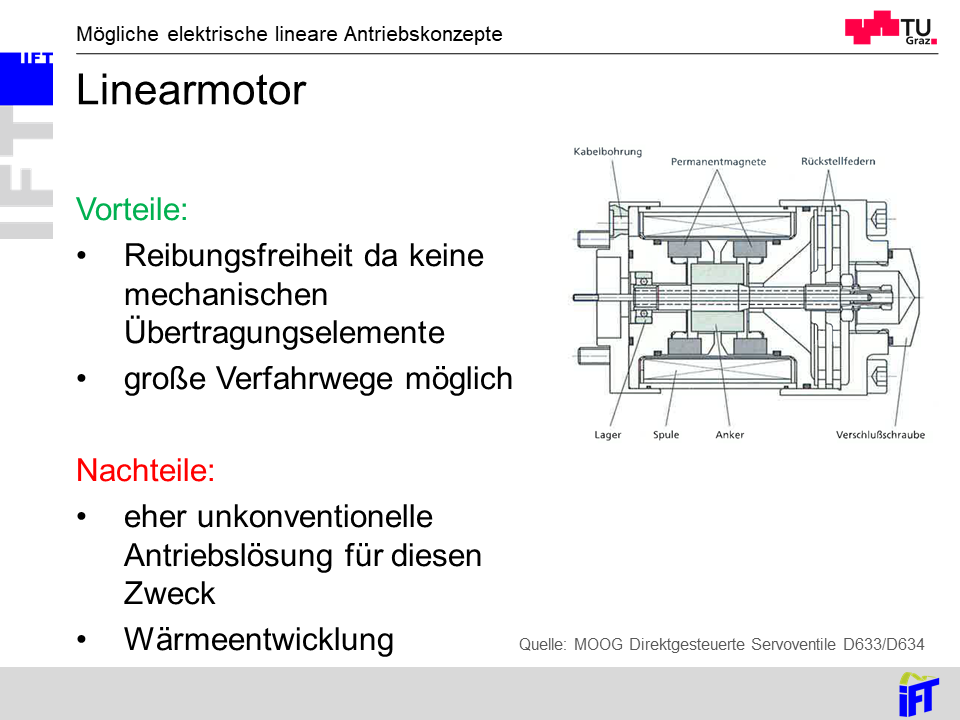
\includegraphics[width=0.7\textwidth]{disc/mech2}
    \caption[Folie]{Folie, Quelle: Eigene Darstellung}
    \label{fig:mech2}
\end{figure}

\begin{figure}[H]
    \centering
    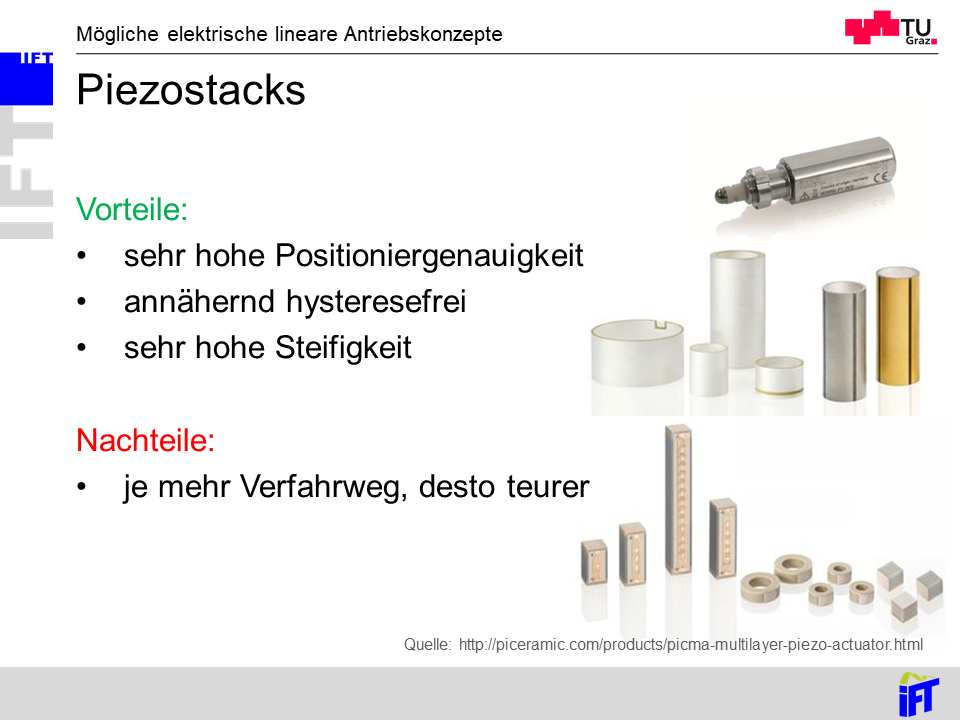
\includegraphics[width=0.7\textwidth]{disc/mech3}
    \caption[Folie]{Folie, Quelle: Eigene Darstellung}
    \label{fig:mech3}
\end{figure}

\begin{figure}[H]
    \centering
    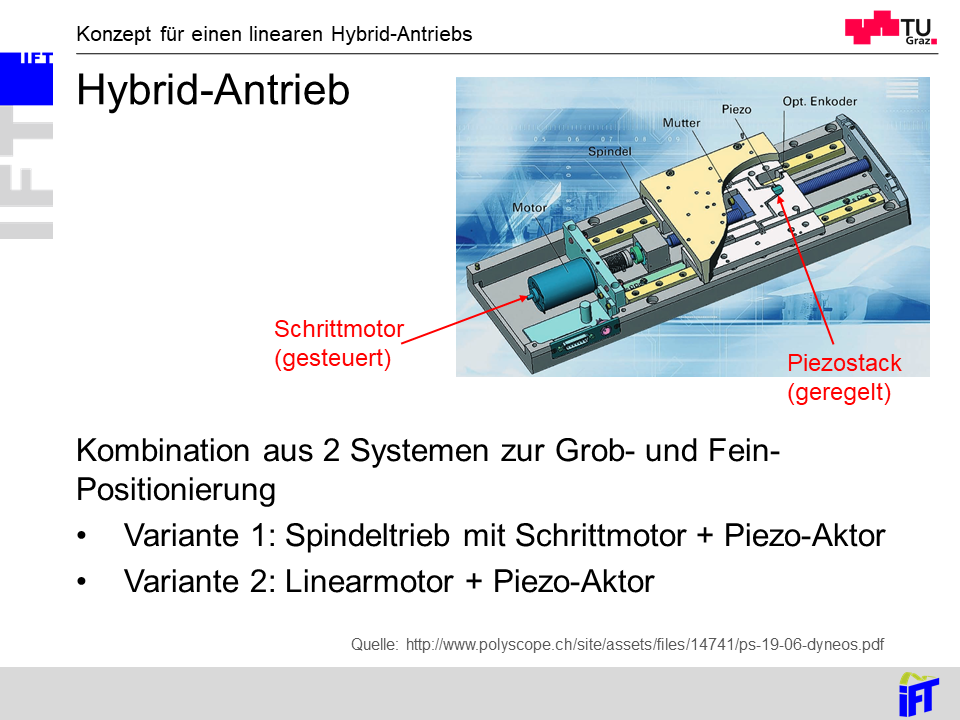
\includegraphics[width=0.7\textwidth]{disc/mech4}
    \caption[Folie]{Folie, Quelle: Eigene Darstellung}
    \label{fig:mech4}
\end{figure}

\begin{figure}[H]
    \centering
    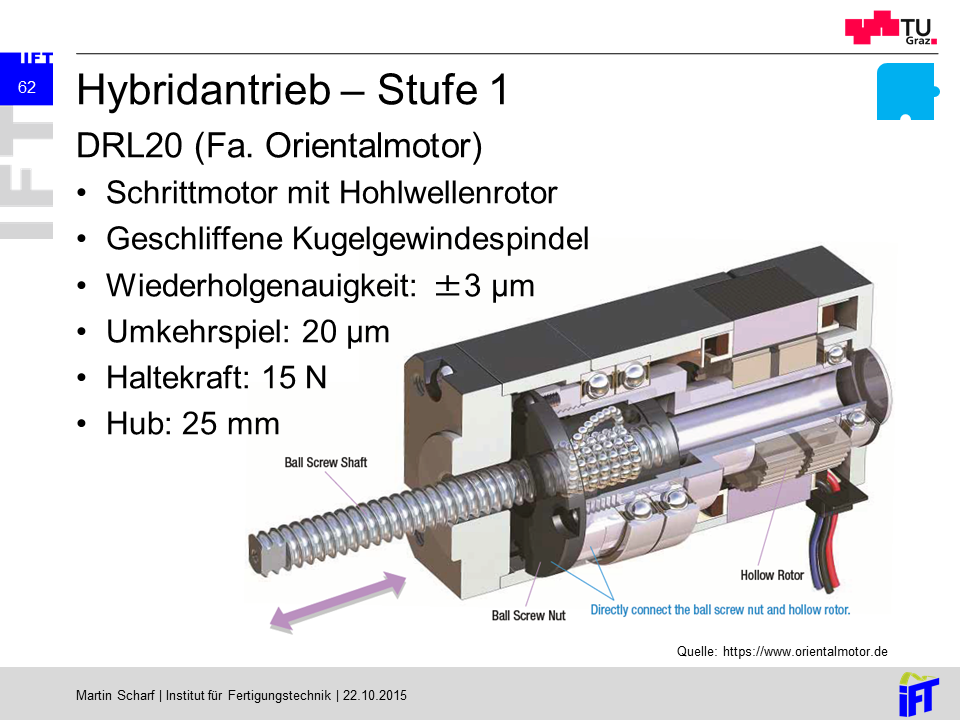
\includegraphics[width=0.7\textwidth]{disc/mech5}
    \caption[Folie]{Folie, Quelle: Eigene Darstellung}
    \label{fig:mech5}
\end{figure}

\begin{figure}[H]
    \centering
    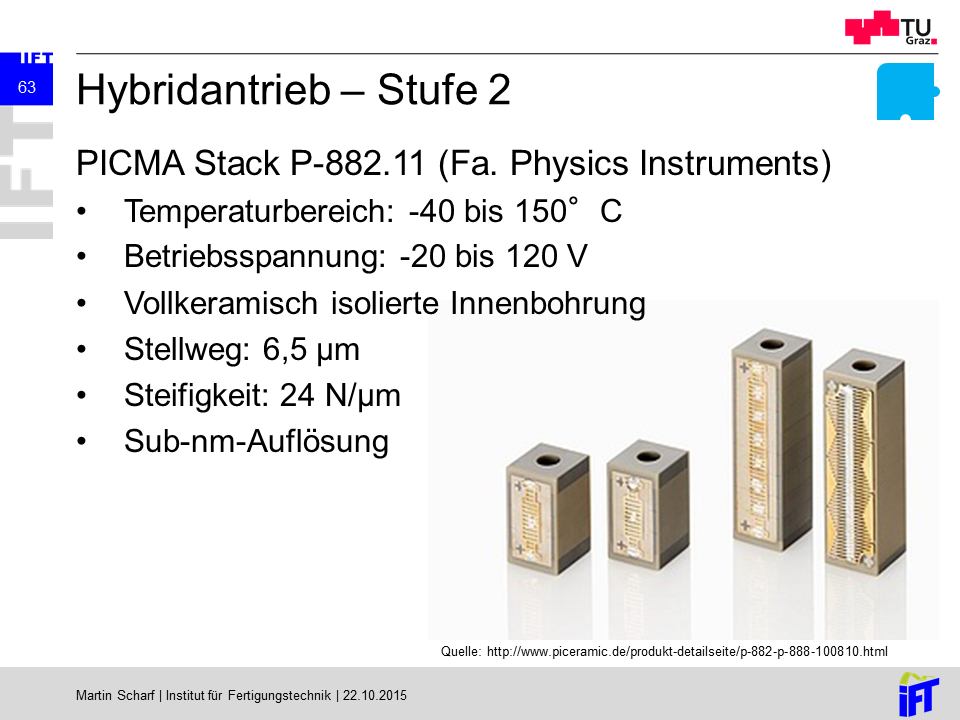
\includegraphics[width=0.7\textwidth]{disc/mech6}
    \caption[Folie]{Folie, Quelle: Eigene Darstellung}
    \label{fig:mech6}
\end{figure}

\begin{figure}[H]
    \centering
    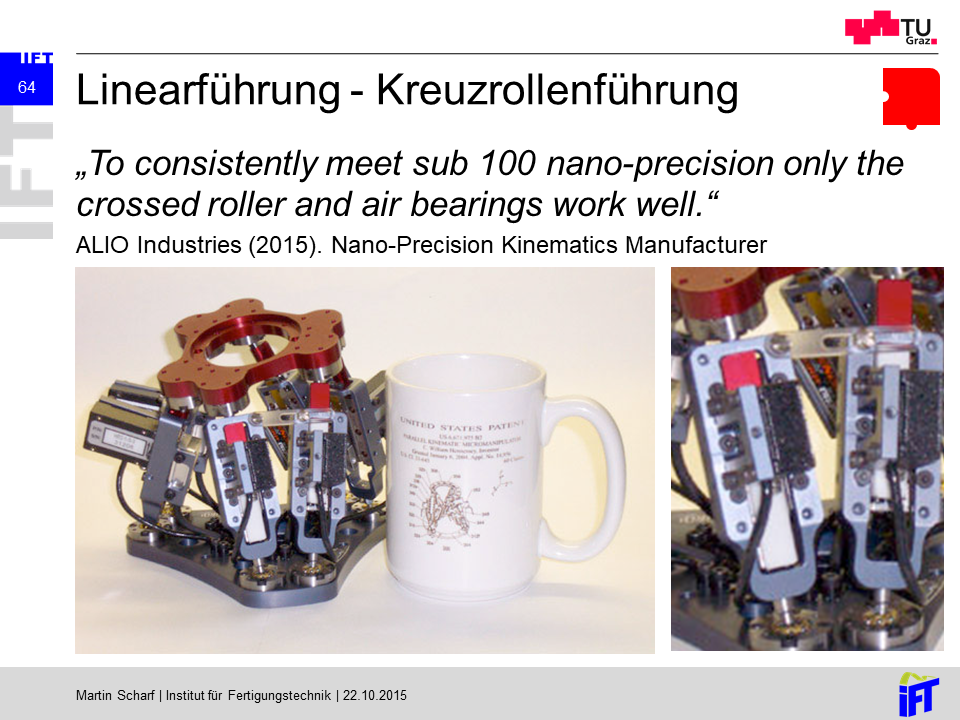
\includegraphics[width=0.7\textwidth]{disc/mech7}
    \caption[Folie]{Folie, Quelle: Eigene Darstellung}
    \label{fig:mech7}
\end{figure}

\begin{figure}[H]
    \centering
    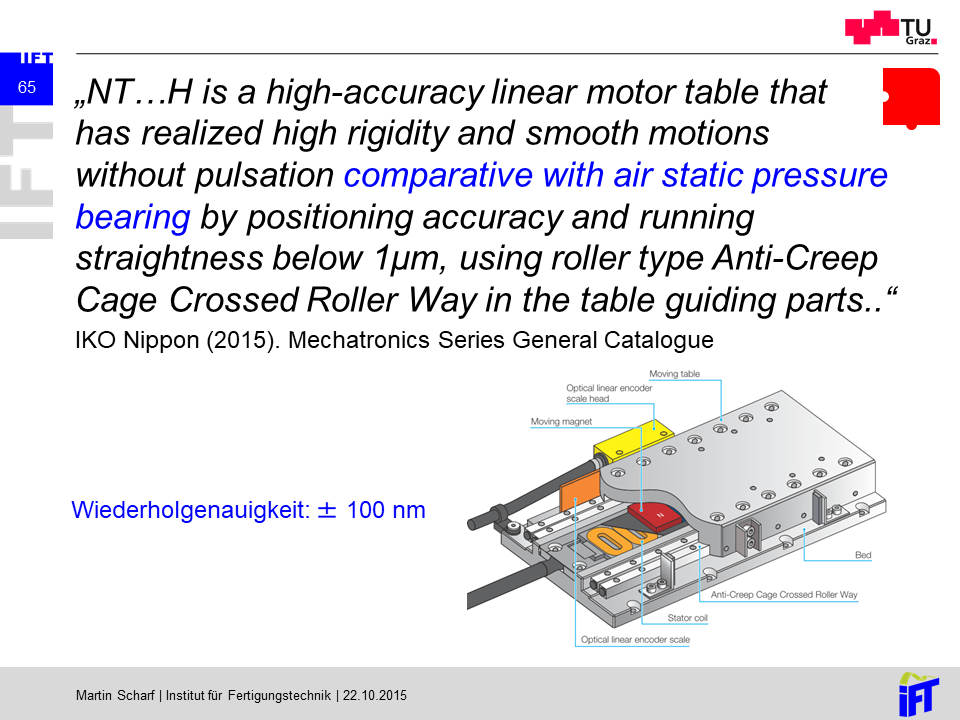
\includegraphics[width=0.7\textwidth]{disc/mech8}
    \caption[Folie]{Folie, Quelle: Eigene Darstellung}
    \label{fig:mech8}
\end{figure}

\begin{figure}[H]
    \centering
    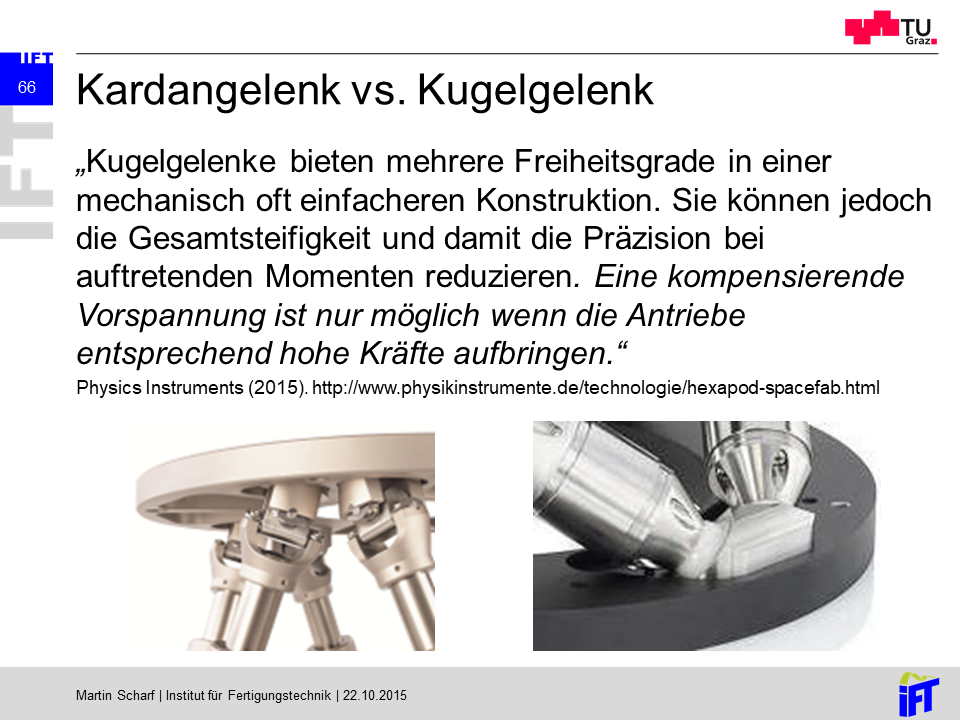
\includegraphics[width=0.7\textwidth]{disc/mech9}
    \caption[Folie]{Folie, Quelle: Eigene Darstellung}
    \label{fig:mech9}
\end{figure}

\begin{figure}[H]
    \centering
    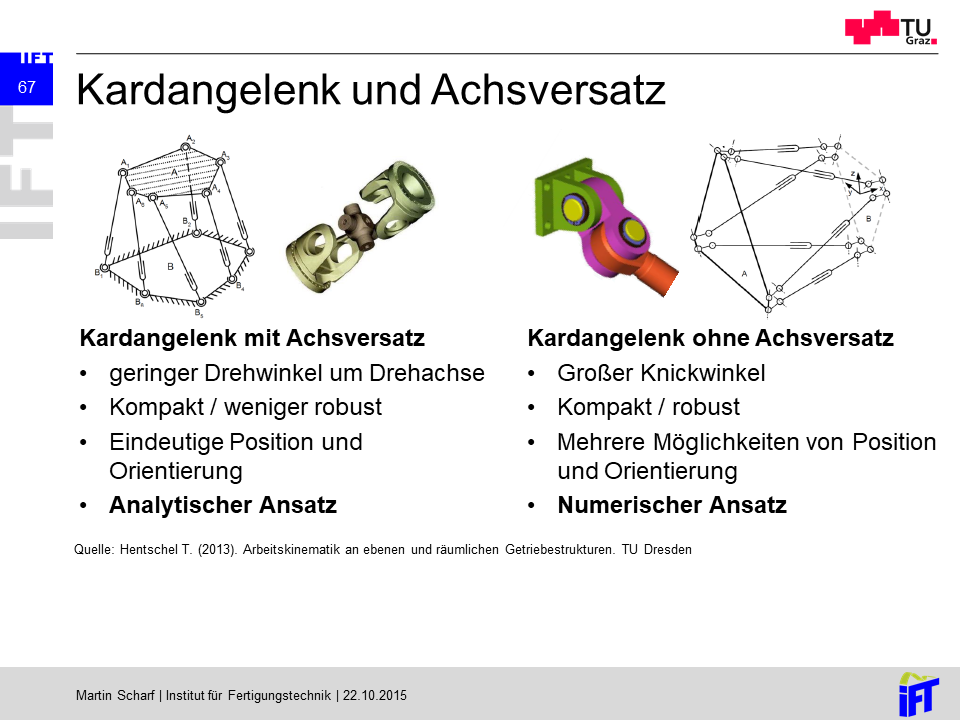
\includegraphics[width=0.7\textwidth]{disc/mech10}
    \caption[Folie]{Folie, Quelle: Eigene Darstellung}
    \label{fig:mech10}
\end{figure}

\begin{figure}[H]
    \centering
    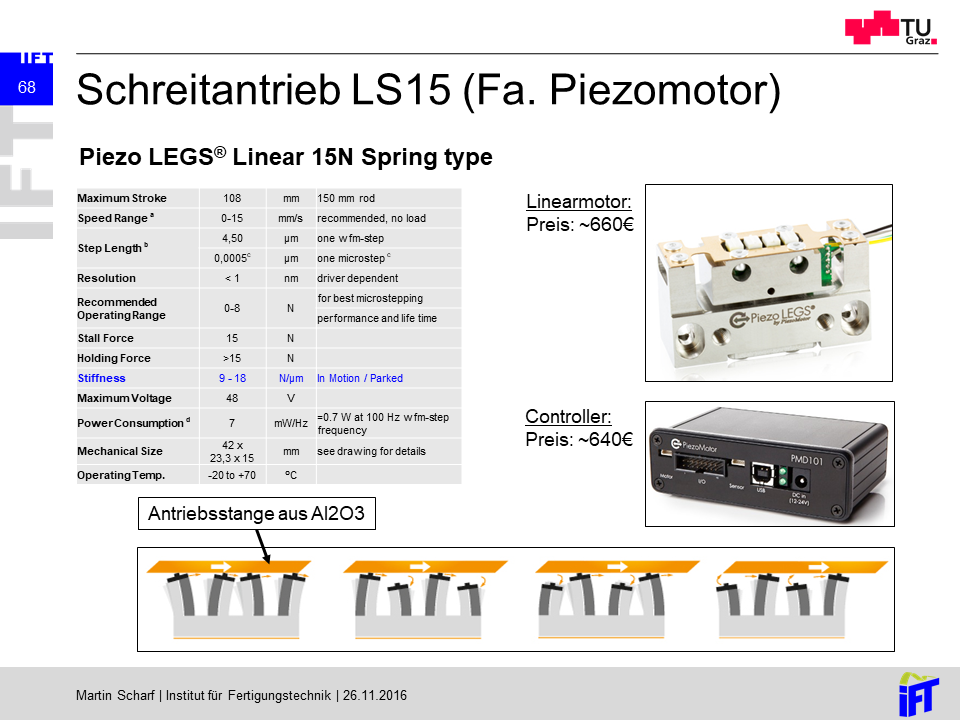
\includegraphics[width=0.7\textwidth]{disc/mech11}
    \caption[Folie]{Folie, Quelle: Eigene Darstellung}
    \label{fig:mech11}
\end{figure}